% !Mode:: "TeX:UTF-8"
% !TEX program  = xelatex
\documentclass[a4paper]{article}
\usepackage{amsmath}
\usepackage{amssymb}
\usepackage{ctex}
\usepackage{graphicx}
%\usepackage{braket}
\usepackage[european]{circuitikz}
\usepackage{multirow}
\usepackage{geometry}
\usepackage{float}
\geometry{left=2.5cm,right=2.5cm,bottom=2.5cm,top=2.5cm}
\title{物理化学实验15: 流动法测定$\gamma-Al_2O_3$小球催化乙醇脱水的催化性能}
\author{XXX\quad 123456789\quad 化学化工学院}
% \date{\today}
\begin{document}
\maketitle
%%\tableofcontents
%%\bibliographystyle{unsrt}
\section{实验目的}
\begin{enumerate}
\item 掌握流动法测定乙醇脱水反应速率常数和活化能的方法.
\item 评价$\gamma - Al_{2}O_{3}$小球催化乙醇脱水的催化性能.
\item 掌握气相色谱在线分析方法, 使用校正面积归一伐进行定量分析.
\end{enumerate}

% \secction{预习要求}
% \begin{enumerate}
% \item 了解流速计, 流量计, 稳压, 稳流阀等的原理和使用方法.
% \item 了解流速法测定催化剂性能的特点和实验方法.
% \item 了解气相色谱分析原理和仪器基本构造.
% \end{enumerate}

\section{实验原理}
\subsection{催化剂的定义}
根据IUPAC于1981年提出的定义: 催化剂是一种能改变反应速率
但不改变该反应的标准吉布斯自由能的物质. 涉及催化剂的反应称为催化反应. 
催化剂不能改变热力学平衡却能影响反应进程达到平衡的速度.
\subsection{催化剂性能评价}
评价催化剂的性能主要有以下几个指标:
\begin{enumerate}
\item 转化率=已经转化的反应物的物质的量 / 反应物起始的物质的量 $\times 100\%$
\item 选择性=转化为目标产物的反应物的物质的量 / 已经转化的反应物的物质的量 $\times 100\%$
\item 收率=转化为目标产物的反应物的物质的量 / 反应物起始的物质的量 $\times 100\%$
\end{enumerate}
\par
另外, 催化剂的活性还可以用``时空收率''表示, 即单位时间内单位体积(或质量)
催化剂上得到的目标产物的量. 需要注意的是, 在表述催化剂的性能时, 还要说明
催化剂活性测定的条件, 如反应温度, 压力, 空速及反应原料组成等.
\subsection{催化剂性能测定方法}
工业上, 依据生产过程的特点, 生产装置可分为连续反应装置和间歇反应装置. 
相应地, 实验室评价催化剂性能时, 可以用连续流动反应器(流动法)
或者釜式反应器(静态法). 实验室用于流动法测定催化剂性能的反应器一般用
耐热玻璃或不锈钢管制成. 催化剂装量一般从不足1毫升至数毫升.
管式反应器依据实验方法的不同又可分为微分反应器和积分反应器.
微分反应器一般要求反应转化率小于$5\%$, 而积分反应器可以在较高转化率下操作.
\par
本次实验采用流动法测定$\gamma-Al_2O_3$小球催化剂乙醇脱水的催化性能,
使用U型管式玻璃反应器, 属积分反应器.
\subsection{流动法}
流动法是使流态反应物不断稳定地流经反应器, 
在反应器催化剂床层中发生反应, 
离开催化剂层反应停止, 然后设法分析产物种类及
数量的一种催化剂活性测定方法. 当催化反应达到稳定状态后, 
反应物的浓度就不随时间变化, 根据反应物区域的体积大小
以及流入和流出反应器的流体的流速和化学组成就可以算出
反应速率. 改变流体的流速或组分的浓度, 就可以测定反应的级数
和速率常数.
\subsection{一级反应速率常数}
如果反应是在管式积分反应器内进行, 催化剂层的总长度是$l$, 
反应管的横截面积是$S$, 反应物只有在催化剂层中才能进行反应. 
假设反应$A\to B$是一级反应, 在反应物接触催化剂之前反应物$A$的浓度
为$c(A_{0})$. 反应物接触到催化剂之后就发生反应, 随着反应物在催化剂
层中通过, 反应物$A$的浓度就逐渐变小, 设在某一小薄层催化剂
$dl$前反应物$A$的浓度为$c_{A}$, 当反应物通过$dl$之后, 浓度变为
$c_{A}-dc_{A}$, 如下图所示.
\begin{figure}[!h]
	\centering
	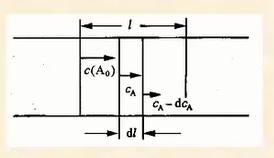
\includegraphics[width=0.30\paperwidth]{fig/mechanics.png}\\
	\caption{流动反应示意图}
\end{figure}
\par
如果是在静止系统, 则一级反应的动力学公式如下, 式中$r$为反应速率, 
$k_{T}$为反应速率常数.
\begin{equation}
r = -\frac{dc_{A}}{dt} = k_{T}c_{A}
\end{equation}
\par
在流动系统中反应物是按稳定的流速流过催化剂层的, 
流速(单位时间内流过的体积)为$F$, 在一小层催化剂内, 
反应物与催化剂接触的时间为$dt$, 则
\begin{equation}
dt = \frac{dV}{F}
\end{equation}
式中, $dV$为一个$dl$薄层催化剂的体积, 而
\begin{equation}
dV = Sdl
\end{equation}
将上述两式带入(1)式可得
\begin{equation}
-\frac{dc_{A}}{c_{A}}=k_{T}\frac{S}{F}dl
\end{equation}
对上式积分, $c_{A}$的积分区间为$c_{0}$到$c$, $l$的
积分区间为$0$到$l$(假设反应前后体积没有变化), 整理可得
下式, 即为稳定流动系统积分反应器中一级反应速率常数表达式.
\begin{equation}
k_{T} = \frac{F}{Sl}\ln\frac{c_{0}}{c}
\end{equation}
\par
在本实验的反应温度下乙醇呈气态, 反应物为乙醇和$N_{2}$
的混合气体, 由于反应压力不高, 反应物近似以理想气体处理. 设
$n_{A}$为单位时间加入乙醇的物质的量$n_{B}$与载气$N_{2}$的
物质的量$n_{D}$的和, 则有:
\begin{equation}
F = \frac{n_{A}RT}{P}
\end{equation}
其中, $F$为反应温度$T$和反应压力$P$下的流速. 反应管中装填的
催化剂体积为$V_{0}$, 则有:
\begin{equation}
Sl = V_{0}
\end{equation}
根据转化率的定义, 乙醇转化率$x = \frac{c_{0}-c}{c_{0}}$, 则:
\begin{equation}
\frac{c_{0}}{c} = \frac{1}{1-x}
\end{equation}
代入式(5)可得, 
\begin{equation}
k_{T} = \frac{n_{A}RT}{PV_{0}}\ln\frac{1}{1-x}
\end{equation}
式中, 
\begin{enumerate}
	\item[] $k_{T}$为乙醇脱水催化反应速率常数
	\item[] $n_{A} = n_{B} + n_{D}$
	\item[] $n_{B}$为单位时间进入反应器的乙醇的物质的量
	\item[] $n_{D}$为单位时间进入反应器的$N_{2}$的物质的量
	\item[] $x$为反应温度$T$下的乙醇转化率
	\item[] $T$, $P$分别为反应条件下的温度和压力
\end{enumerate}
\subsection{乙醇脱水反应}
乙醇在$\gamma-Al_2O_3$小球催化剂上发生脱水反应, 主要产物与反应温度
密切相关. 温度低时, 乙醚为主要产物, 随着温度的升高, 
乙烯的选择性逐渐升高, 并成为主要产物, 另外会有极少量的乙醛生成. 
本实验反应温度为$200-250^\circ$C, 乙醚为主要产物. 
乙醇脱水反应方程式如下: 
\begin{enumerate}
	\item $C_{2}H_{5}OH \to C_{2}H_{4} + H_{2}O$
	\item $2C_{2}H_{5}OH \to C_{2}H_{5}OC_{2}H_{5} + H_{2}O$
\end{enumerate}
\par
在较低的反应温度下, 由于主要生成乙醚, 
可以近似认为反应前后体系体积不变, 即气相流速不变. 
另外, 假定反应(1) 和反应(2) 为平行反应, 并假定二者皆为一级反应, 
乙醇脱水生成乙烯和乙醚的速率常数分别为$k_{T1}$和$k_{T2}$, 生成
乙烯和乙醚的选择性分别为$s_{1}$和$s_{2}$, 忽略乙醇脱氢生成乙醛
的量, 则$s_{1}+s_{2}\approx 1$, 对于平行一级反应,
\begin{equation}
	\begin{aligned}
		\frac{k_{T1}}{k_{T2}} &= \frac{s_{1}}{s_{2}}\\
		k_{T} &= k_{T1} + k_{T2}\\
	\end{aligned}
\end{equation}
可得:
\begin{equation}
	\begin{aligned}
		k_{T1} &= s_{1}k_{T}\\
		k_{T2} &= s_{2}k_{T}\\
	\end{aligned}
\end{equation}
\subsection{乙醇脱水催化反应装置}
流动法测定$\gamma-Al_2O_3$小球催化乙醇脱水的催化性能(色谱法)
的实验装置主要由以下几个部分构成:
\begin{enumerate}
\item \textbf{原料进样单元}: 乙醇进样泵, $N_{2}$流量控制系统
\item \textbf{反应单元}: 反应炉及温度控制和测量仪表
\item \textbf{色谱分析单元}: 反应尾气连接气路, 进样阀及气相色谱仪
\item \textbf{数据采集及处理单元}: 色谱工作站及计算机
\end{enumerate}
\subsection{色谱定量方法}
目前常用的色谱定量分析方法主要有三种: 面积归一法, 内标法和外标法.
本次实验采用面积归一法.
\par
由于不同组分在检测器上的响应值不同, 故需对峰面积采用校正因子校正, 
可称为校正面积归一法, 计算公式为:
\begin{equation}
n_{i}\% = \frac{f_{Mi}A_{i}}{\sum f_{Mi}A_{i}}\times 100\%
\end{equation}
式中, $n_{i}\%$, $f_{Mi}$和$A_{i}$分别为待测组分的摩尔百分浓度, 
摩尔校正因子, 峰面积. 具体组分的摩尔校正因子在实验室的黑板上列明.
\par
面积归一法的优点是简便, 受操作条件影响较小, 但要求所有组分都能被
色谱检测出, 因此有一定的局限性和误差.
\section{仪器与药品}
\begin{enumerate}
    \item \textbf{仪器}: 微型固定床反应装置, 气相色谱仪, 气源, 电脑,
	检漏用毛笔,肥皂液, 微量进样器($1\mu L$和$100\mu L$), 直尺, 表面皿, 
	乙醇试剂, 样品筛($20 -- 40$目), 微量注射泵控制器, 计时器,
	保温控制仪(加热带), 保温控制仪(电炉), 温度显示器(电炉), 微量注射泵主体, 
	U型反应管, 电炉, 转子流量计, 压力表, 皂膜流量计, 普通六通阀(接填充柱), 
	气动自动进样阀(接毛细管柱), 三通
	\item \textbf{仪器}: 氮气钢瓶(黑色), 总阀, 减压阀, 表头(总压), 表头(输出压力),
	空气发生器, 氢气发生器(保证试验时水量处于上下限之间)
    \item \textbf{药品}: $\gamma-Al_2O_3$小球催化剂, 石英砂, 乙醇
\end{enumerate}
\section{实验注意事项}
\begin{enumerate}
\item 系统必须不漏气
\item 在实验过程中热电偶的位置必须固定不变
\item 由于使用气相色谱分析尾气组成, 所以尾气管路必须保温, 
确保加热带开关打开
\item 氮气的流速以及乙醇的进样速度在实验过程中必须保持稳定
\item 实验过程中要勤观察, 尤其要注意反应温度波动情况
\end{enumerate}
\section{实验步骤}
详见``流动法测定$Al_2O_3$小球催化剂乙醇脱水的催化性能修改后步骤''文档.
% \section{实验步骤}
% \subsection{装样}
% \begin{enumerate}
% \item 一手扶住U型反应管上端, 另一只手顺时针松开螺帽, 
% 取下反应管. 取下O型圈和螺帽, 将管内的石英砂和催化剂倒入催化剂回收瓶, 
% 清洗反应管(可用PVC气路管作为毛刷), 用去离子水荡洗, 放入$120^\circ$C烘箱干燥.
% \item 称取$50mg(\pm 1mg)$的$\gamma-Al_2O_3$小球催化剂, 
% 在干燥后的U型反应管口套上漏斗, 加入称取的催化剂, 抖动, 使催化剂均匀分布于U型
% 管底.
% \item 分别称取两份$0.4g 8 -- 16$目石英砂, 放入反应管两端.
% \item 分别套上螺帽和O型圈, 将反应管接入反应装置, 逆时针旋紧(但不要产生扭力).
% \end{enumerate}
% \subsection{活化}
% \begin{enumerate}
% \item 在减压阀处于关闭状态时打开氮气钢瓶总阀, 顺时针转动减压阀旋钮, 
% 调节出口压力为$0.3$MPa. 
% \item 打开控制面板上的开关阀, 通过稳压阀旋钮, 
% 调节压力指示为$0.1$MPa. 调节调流阀旋钮, 使转子流量计指示约为
% $50mL \cdot min^{-1}$.
% \item 检漏, 为了防止肥皂水流入电炉, 用吸水纸包住反应管, 
% 用蘸有肥皂液的毛笔涂抹反应管与螺帽的接口处, 
% 如果有气泡产生, 说明此处漏气, 用吸水纸擦干螺帽后进一步旋紧. 
% 再次检漏, 若再次漏气则需要更换O型圈.
% \item 擦干反应管后, 调整热电偶的位置, 
% 使测量端与反应管底部齐平. 调节升降台, 使反应管处于
% 电炉之中. 用直尺测量螺帽口与电炉口之间的距离, 控制到$4 -- 5$cm左右. 
% 用保温带盖住电炉口处的空隙.
% \item 打开控制面板上电源开关, 设置电路温度控制参数(按SET键两次再按左键进入设置界面), 
% 按照温度--时间--温度设置每一段的程序升温条件. 设置完毕, 等待仪器
% 自动进入工作界面. 
% \item 同时按住上下键直至出现RUN.
% \end{enumerate}
% \subsection{气相色谱仪设置}
% \begin{enumerate}
% \item 打开气相色谱仪柱箱舱门, 查看是否已正确安装SE-54毛细管色谱柱, 
% 关闭舱门.
% \item 打开色谱仪电源开关和电脑中NetChrom在线工作站.
% \item 点击左下角图标连接对应的色谱仪, 右上角界面会显示当前色谱的参数
% \item 设置进样$A$为$120^\circ$C, 柱箱$60^\circ$C, FID$250^\circ$C, 
% 气动阀$120^\circ$C, 停止时间$4.9min$, 满屏时间$5min$, 上限800, 下限0. 
% 在``系统->选项->操作''中设置文件保存位置.
% \item 点击开始控温, 打开氢气和空气发生器开关, 通过色谱顶部旋钮, 按3键调节载气$N_{2}$
% 流速为$2mL\cdot min^{-1}$, 对应a柱压力为35kPa, 分流比调至20左右. 按4键可以调节FID检测器参数, 
% 氢气流速为$30mL\cdot min^{-1}$, 空气流速为$300mL\cdot min^{-1}$. 按7键进入采集参数设置界面, 
% 进样次数设置为3次, 间隔时间为$5min$, 按SET键保存退出设置状态.
% \item 按下键进入$No. 5$界面, 将第一排参数设置为$0.02$和$1$, 表示$0.02$min时气动阀
% 采样, $1min$时分析采集样品.
% \item 检测点火是否成功.
% \end{enumerate}
% \subsection{反应}
% \begin{enumerate}
% \item 打开气路管保温带加热开关(位于气路面板右侧), 控制温度设置为$120^\circ$C, 
% 将气路的三通调至与皂膜流量计相通的位置, 轻轻挤压皂膜流量计
% 底部的滴帽, 产生成串气泡以润湿管壁, 直至气泡能从流量计管壁冒出. 
% 快速挤压滴帽, 产生单个皂膜, 在皂膜通过第一个刻度线时开始计时, 
% 通过第二个刻度线时停止计时, 通过调流阀调节流速, 使皂膜流量计流速
% 为$50mL\cdot min$.(需要准确记录流速)
% \item 将三通转至连接尾气位置, 打开微量注射泵开关, 设置原料液进样参数. 
% 选择流量->上海高鸽$100\mu L$注射器, 设置单位为$\mu L$, 分配液量$30$, 
% 灌注时间为$15min$.
% \item 待温度恒定后可以开始反应.
% \item 进样器取$80\mu L$乙醇, 排出气体, 将进样器插入进样口, 
% 将进样器固定到微量注射泵的卡槽中, 固定针筒. 调节注射泵挡板至
% 正好顶住进样器推杆, 按启动键启动微量注射泵开始进样. 
% \item 按色谱控制面板上的start键开始气相色谱分析程序.
% \item 关闭微量注射泵, 色谱仪, 观察反应后催化剂的颜色变化.
% \end{enumerate}

\section{拓展实验设计}
升高反应温度至$170^\circ$C, 使生成乙烯的反应占主导, 无法控制反应前后体积近似不变.
\section{实验现象记录}
\begin{enumerate}
	\item 反应后催化剂的颜色变化
\end{enumerate}

\newpage
\section{数据处理}
\begin{enumerate}
\item 根据$n_{B} = \frac{q_{C_{2}H_{5}OH}\times \rho_{C_{2}H_{5}OH}}{M_{C_{2}H_{5}OH}}$
求出单位时间通入反应体系乙醇的物质的量$n_{B}$, 式中$q_{C_{2}H_{5}OH}$, $\rho_{C_{2}H_{5}OH}$, $M_{C_{2}H_{5}OH}$
分别为乙醇进样速度, 乙醇在进样温度(室温)时的密度, 乙醇的摩尔质量. 单位时间通入反应体系
$N_{2}$的物质的量$n_{D}$由$q_{n_{2}}P = n_{D}RT$求出, 式中$q_{N_{2}}$为皂膜流量计标定的
载气氮气的流速, $T$, $P$分别为标定时的室温大气压.
\item 根据相关定义求出并正确表示各温度下乙醇的转化率及
生成乙烯和乙醚的选择性, 以及接触时间, 空速, 收率和时空收率.
\item 根据式(9)计算各温度下乙醇脱水催化反应速率常数$k_{T}$.
\item 分别计算各温度下乙醇脱水生成乙烯和乙醚的反应速率常数
$k_{T1}$和$k_{T2}$.
\item 分别以$\ln k_{T1}$和$\ln k_{T2}$对$\frac{1}{T}$作图, 
从直线斜率求出乙醇脱水生成乙烯和乙醚的表观活化能$E_{a1}$和$E_{a2}$.

\begin{table}[H]
	\begin{center}
		\caption{拟合参数}
		\begin{tabular}{l|l|l|l|l|l|l}
			\hline
			$T/^\circ$C&$k_{T}/s^{-1}$&$\frac{1}{T}/K^{-1}$& $k_{T1}/s^{-1}$ & $k_{T2}/s^{-1}$ & $\ln k_{T1}/ln s^{-1}$ & $\ln k_{T2}/ln s^{-1}$\\
			\hline
			$200$&$7.634\times 10^{-1}$&$2.113$ & $1.063\times 10^{-2}$ & $7.523\times 10^{-1}$ &$-4.544$&$-0.2846$\\
			\hline
			$210$&1.447&$2.070$ & $3.191\times 10^{-2}$ & $1.416$ &$-3.445$&$0.3475$\\
			\hline
			$220$&2.322&$2.028$ & $9.713\times 10^{-2}$ & $2.223$ &$-2.332$&$0.7990$\\
			\hline
			$230$&3.543&$1.987$ & $2.661\times 10^{-1}$ & $3.274$ &$-1.324$&$1.186 $\\
			\hline
			$240$&4.361&$1.949$ & $4.830\times 10^{-1}$ & $3.873$ &$-0.7278$&$ 1.354$\\
			\hline
		 \end{tabular}
	\end{center}
\end{table}
\begin{table}[H]
	\begin{center}
		\caption{各温度下的转化率, 选择性和收率}
		\begin{tabular}{l|l|l|l|l|l}
			\hline
			$T^\cdot$C	&乙醇转化率/$\%$	&乙烯选择性/$s_1\%$	&乙醚选择性/$s_2\%$	& 乙烯收率/$Y_1\%$ & 乙醚收率/$Y_2\%$\\
			\hline
			200&11.893 &1.393&98.55&0.170 &	11.718 \\
			\hline
			210&20.953 &2.205&97.80&0.464 &	20.489 \\
			\hline
			220&30.889 &4.184&95.78&1.294 &	29.583 \\
			\hline
			230&42.457 &7.511&92.40&3.192 &	39.228 \\
			\hline
			240&48.678 &11.07&88.81&5.392 &	43.230 \\
			\hline
		 \end{tabular}
	\end{center}
\end{table}
\begin{table}[H]
	\begin{center}
		\caption{各温度下的时空收率}
		\begin{tabular}{l|l|l}
			\hline
			$T^\cdot$C&乙烯时空收率/$mol\cdot min^{-1}\cdot g^{-1}$&乙醚时空收率/$mol\cdot min^{-1}\cdot g^{-1}$\\
			\hline
			200&$1.13\times 10^{-5}$&$8.00\times 10^{-4}$\\
			\hline
			210&$3.15\times 10^{-5}$&$1.40\times 10^{-3}$\\
			\hline
			220&$8.82\times 10^{-5}$&$2.02\times 10^{-3}$\\
			\hline
			230&$2.18\times 10^{-4}$&$2.68\times 10^{-3}$\\
			\hline
			240&$3.68\times 10^{-4}$&$2.95\times 10^{-3}$\\
			\hline
		\end{tabular}
	\end{center}
\end{table}

乙醇液体空速$=\frac{q_{v}(C_{2}H_{5}OH)}{V_{0, cat}} = 
\frac{2.00\times10^{-3}mL\cdot min^{-1}}{0.0501g/0.2222g\cdot cm^{-3}} = 8.87\times10^{-3}min^{-1}$.
\begin{table}[H]
	\begin{center}
		\caption{各温度下的空速与接触时间}
		\begin{tabular}{l|l|l}
		\hline
		$T^\cdot$C &总空速/$min^{-1}$&接触时间/min\\
		\hline
		200		&$3.62\times 10^{2}$	&$2.76\times 10^{-1}$\\
		\hline
		210 	&$3.69\times 10^{2}$	&$2.71\times 10^{-1}$\\
		\hline
		220 	&$3.77\times 10^{2}$	&$2.65\times 10^{-1}$\\
		\hline
		230 	&$3.85\times 10^{2}$	&$2.60\times 10^{-1}$\\
		\hline
		240 	&$3.92\times 10^{2}$	&$2.55\times 10^{-1}$\\
		\hline
		\end{tabular}
	\end{center}
\end{table}
乙醇脱水生成乙烯表观活化能计算,
\begin{figure}[H]
	\centering
	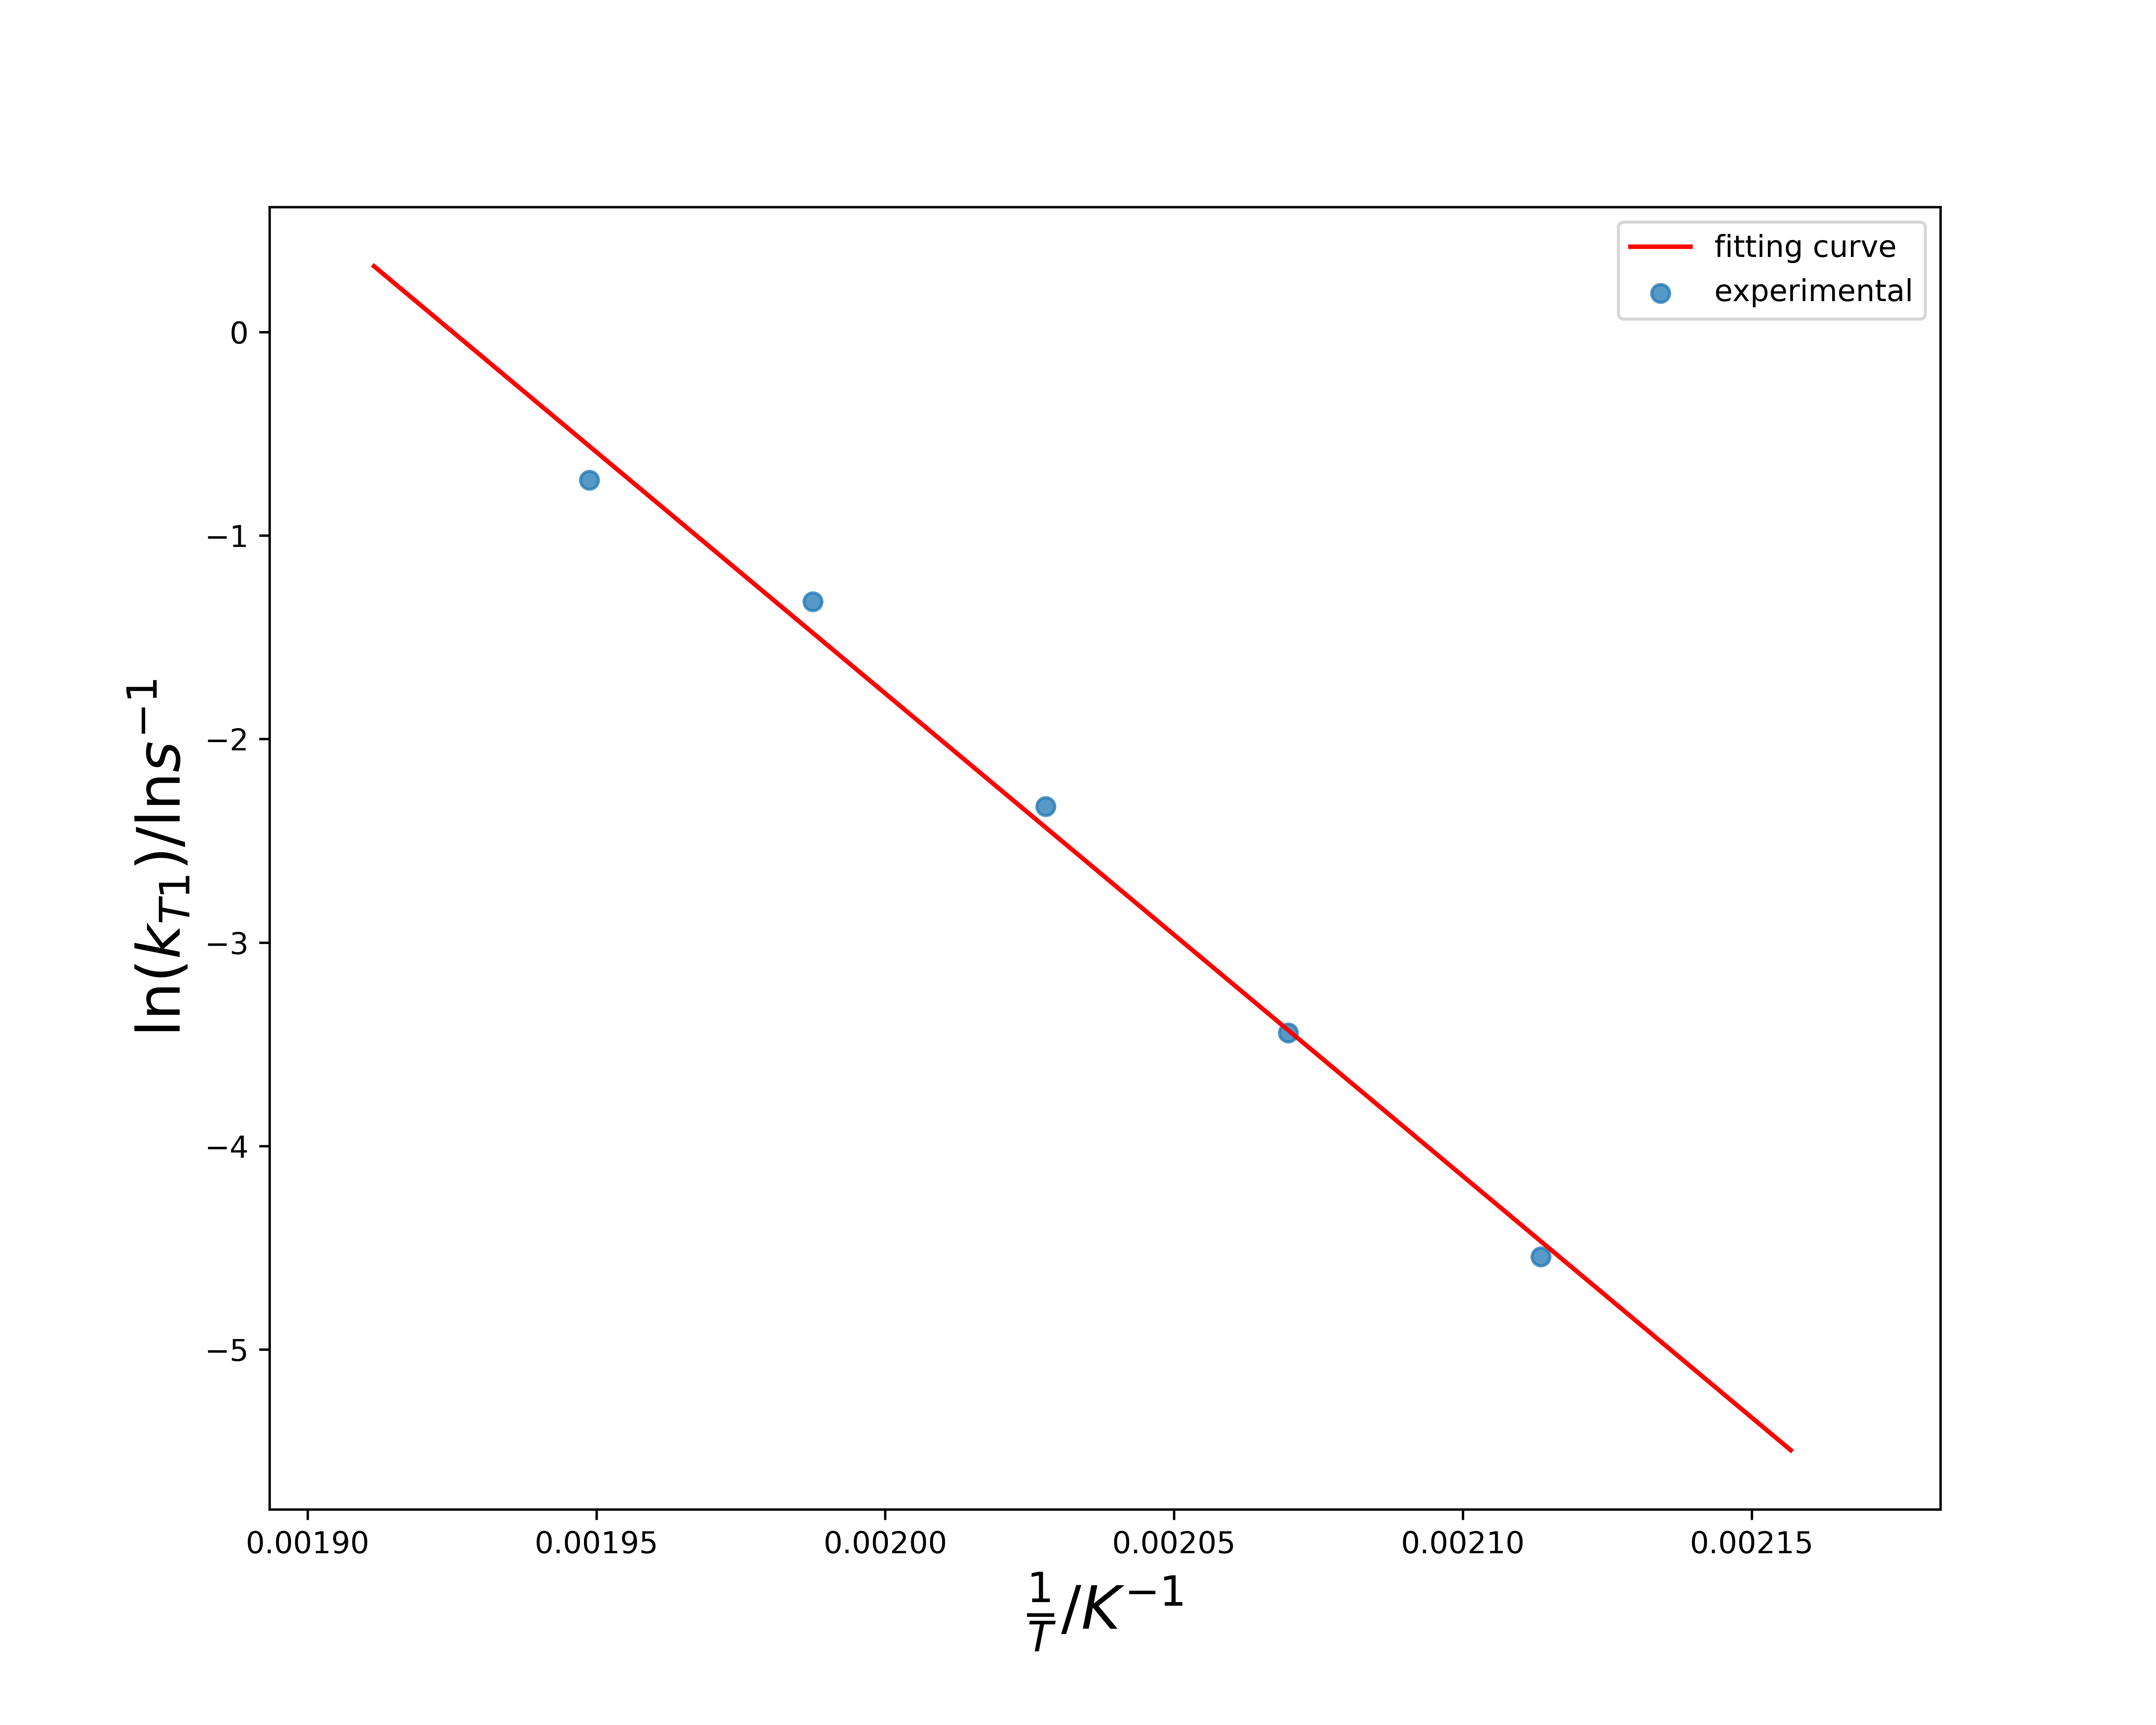
\includegraphics[width=0.50\paperwidth]{fig/kT1.png}\\
	\caption{反应速率常数$\ln(k_{T1})$对温度$\frac{1}{T}$作图}
\end{figure}
最小二乘法一次函数拟合结果如下,
\begin{equation}
	\begin{aligned}
		\ln k_{T1} &= -2.372\times 10^{4} \times \frac{1}{T} + 45.67\\
		E_{a1} &= 2.372\times 10^{4} \times 8.314 J\cdot mol^{-1}\\
		       &= 197.2 kJ\cdot mol^{-1}\\
		R^{2} &= \frac{SSR}{SST} = \frac{\sum{(\hat{k_{T1,i}}-\bar{k_{T1}})^{2}}}{\sum{(k_{T1,i}-\bar{k_{T1}})^{2}}}\\
					&=0.9928\\
	\end{aligned}
\end{equation}
乙醇脱水生成乙醚表观活化能计算,
\begin{figure}[H]
	\centering
	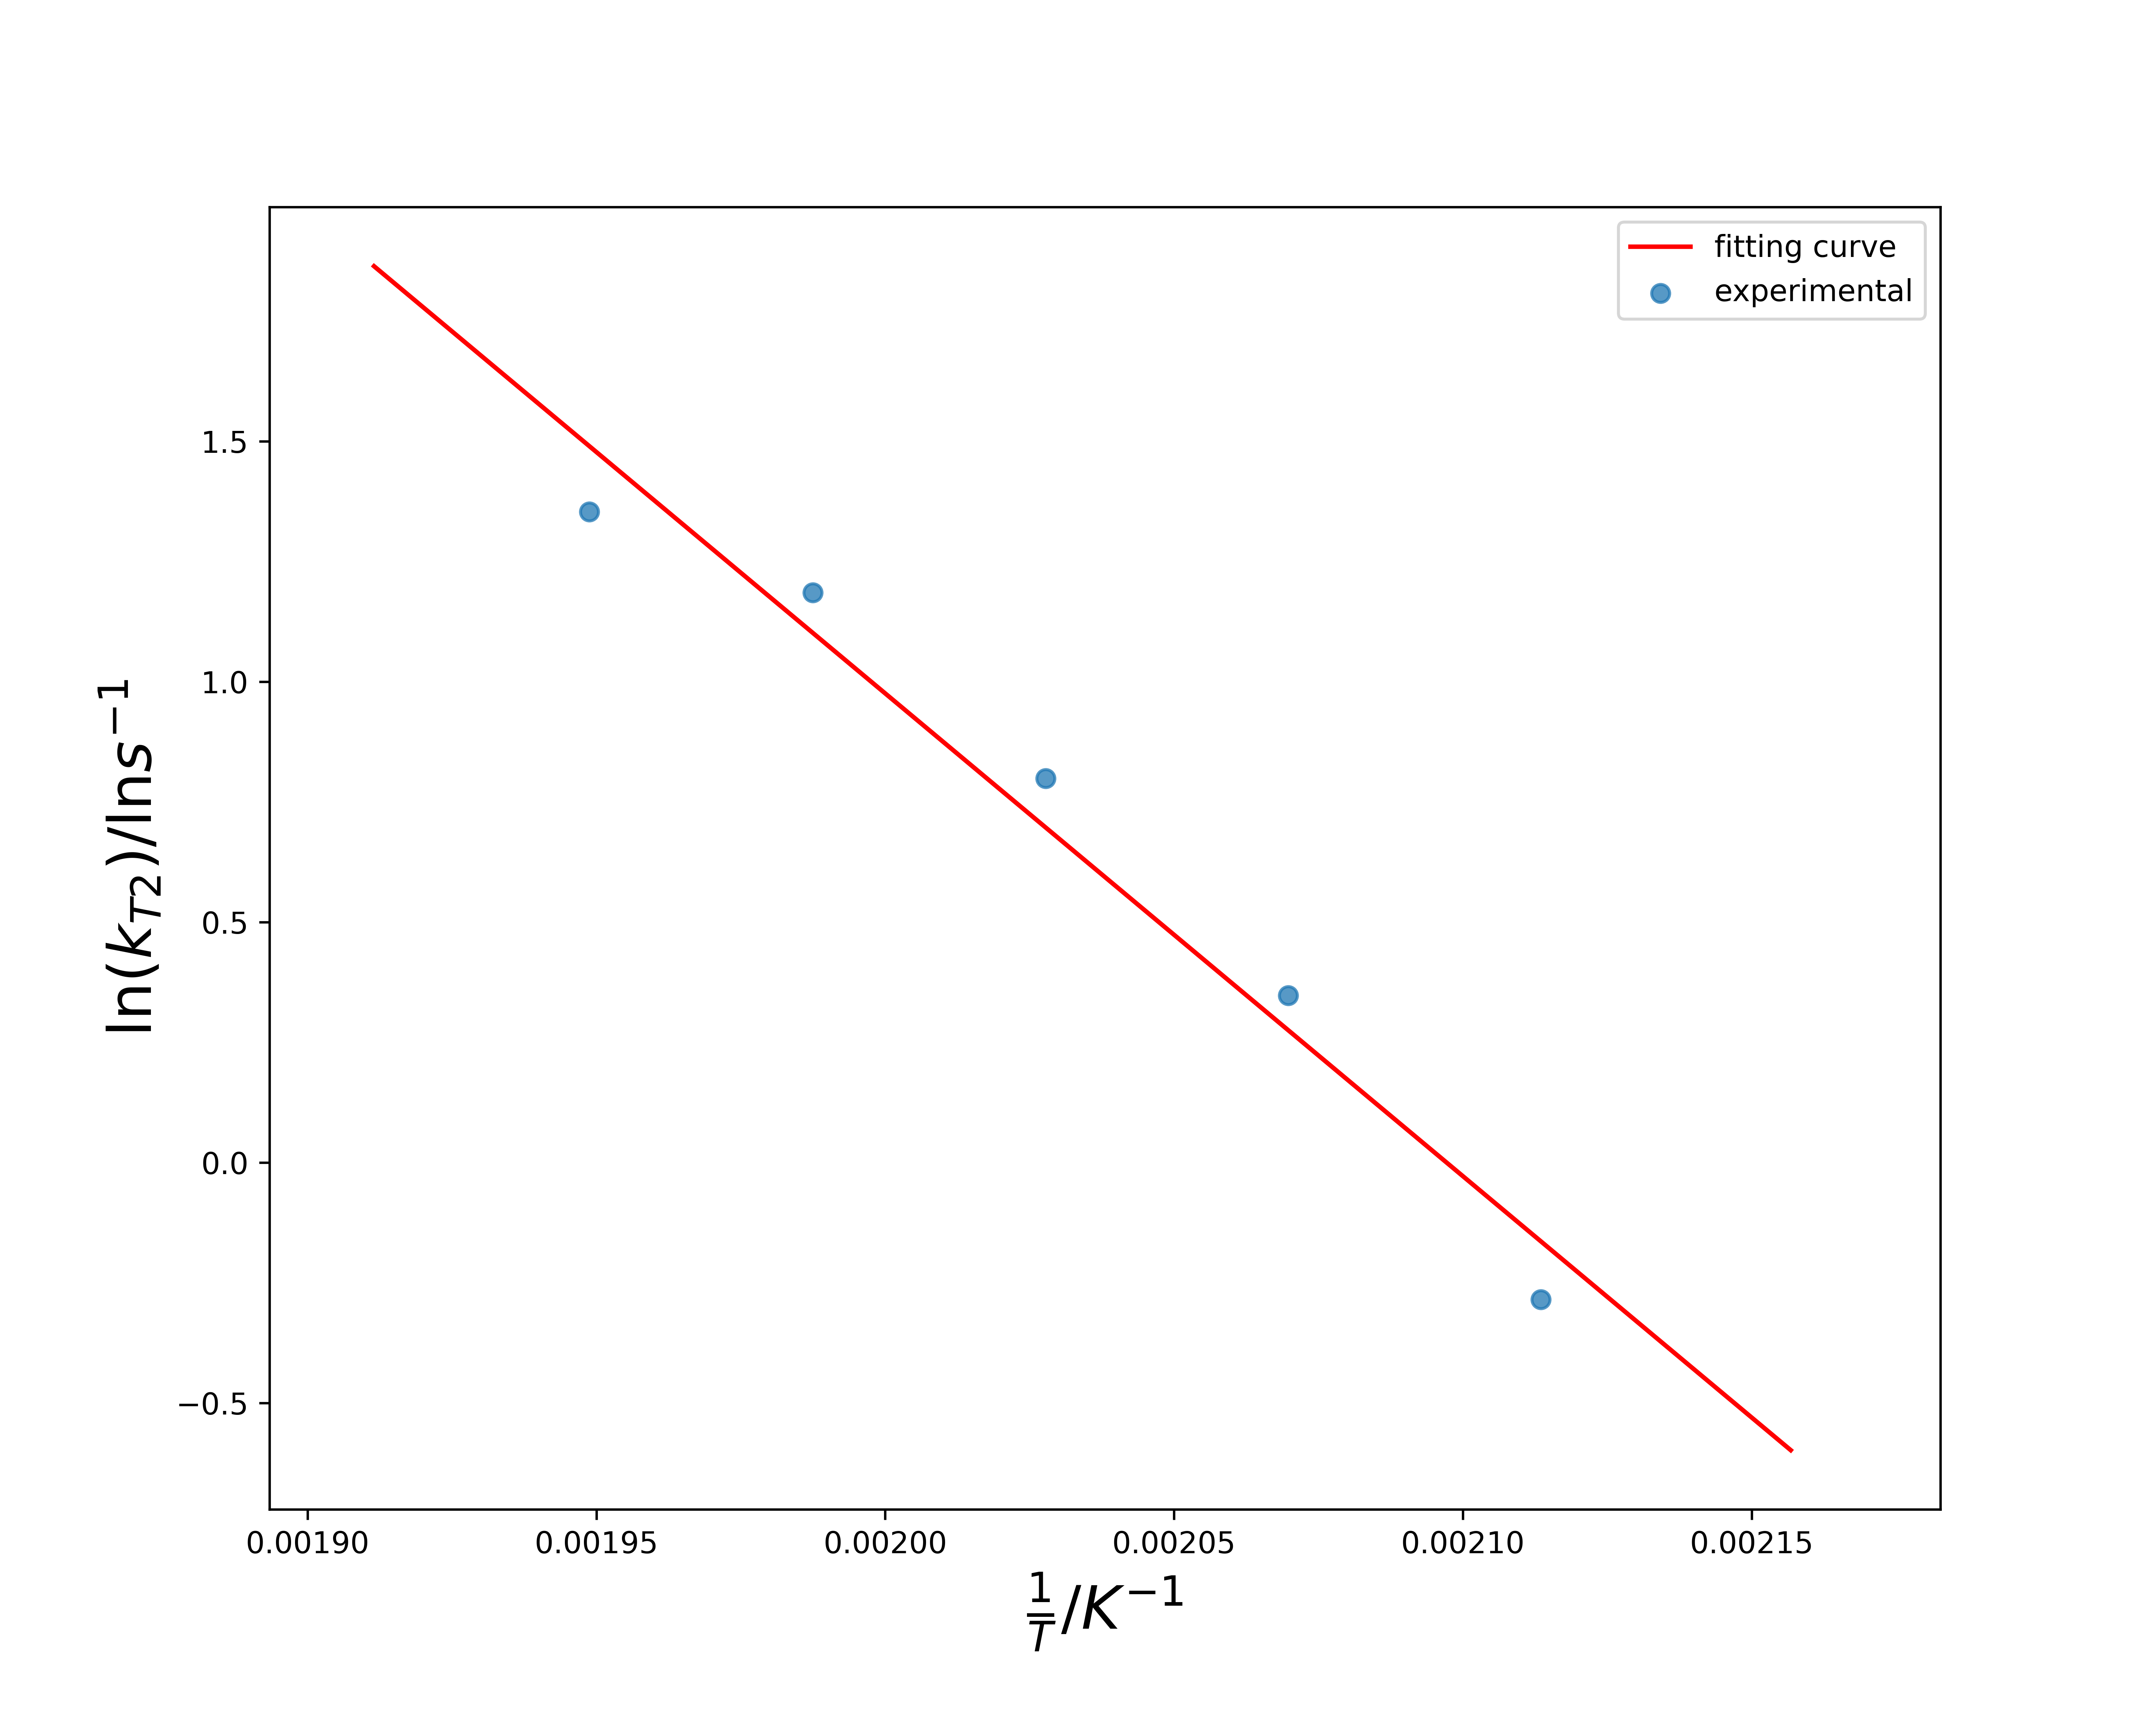
\includegraphics[width=0.50\paperwidth]{fig/kT2.png}\\
	\caption{反应速率常数$\ln(k_{T2})$对温度$\frac{1}{T}$作图}
\end{figure}
最小二乘法一次函数拟合结果如下,
\begin{equation}
	\begin{aligned}
		\ln k_{T2} &= -1.004\times 10^{4} \times \frac{1}{T} + 21.05\\
		E_{a2} &= 1.004\times 10^{4} \times 8.314 J\cdot mol^{-1}\\
				&= 83.47 kJ\cdot mol^{-1}\\
		R^{2} &= \frac{SSR}{SST} = \frac{\sum{(\hat{k_{T2,i}}-\bar{k_{T2}})^{2}}}{\sum{(k_{T2,i}-\bar{k_{T2}})^{2}}}\\
					&=0.9683\\
	\end{aligned}
\end{equation}


\end{enumerate}
\newpage
\section{思考题与讨论}
\begin{enumerate}
	\item 本次实验中转子流速计和皂膜流速计各有什么作用?\\
	转子流速计可以粗略的测量气路中的$N_{2}$流速, 
	但精确流速需要用皂膜流量计测定; 并且转子流速计不能直接测定流速, 
	需要用皂膜流量计校正.
	\item 流动法测定催化剂活化能的特点是什么? 有哪些注意事项?\\
	反应物可以不断稳定的流经反应器, 生成物连续稳定地流出反应器.
	实验中需要控制反应过程中反应条件(温度/压力/流速等)一致.
	\item 如何通过改变反应条件, 控制平行反应的选择性?\\
	由实验结果可知, 乙醇脱水生成乙烯的表观活化能比生成乙醚的表观活化能高, 
	因此升高反应温度, 乙烯选择性增加; 由反应方程式可知, 增加反应压力会抑制
	生成脱水生成乙烯. 
	\item 从阿伦尼乌斯公式来测定表观活化能时, 需要对反应有何控制?\\
	$lnk = -\frac{E_{a}}{RT} + b$, 反应速率常数的对数与温度的倒数作图, 通过斜率计算
	得到表观活化能, 因此需要保证温度的测量和对应反应速率常数的计算是可靠的. 反应速率常数
	除了受温度影响外, 其他环境因素如催化剂的种类/质量/是否中毒, 压力, 反应物流入体系的速度和
	生成物移除反应体系的速度, 这些因素反应在常数$b$中, 反应过程中都需保持恒定.
\end{enumerate}
\section{误差分析}
\begin{enumerate}
	\item $200^\circ$C第一组数据弃用是因为反应刚开始时间较短未达到平衡; 
	\item 从$210^\circ$C开始每一个温度乙醇都在未检测状态下反应5min, 
	由于$210^\circ$C时没有将微量注射泵设置的时间改为20min, 因此导致$210^\circ$C
	测得的最后一组数据没有乙醇进样, 出现错误.
	\item 反应温度高时, 电炉温度显示器温度变化较大, 由于$250^\circ$C下测得的第一组数据
	和另两组数据差距较大, 因此不计入平均值计算.
\end{enumerate}
\newpage
\section{原始数据记录}
\begin{table}[H]
	\begin{center}
		\begin{tabular}{l|l}
			\hline
			室温/$^\circ$C & 大气压/kPa\\
			\hline
						   &           \\
			\hline
		 \end{tabular}
	\end{center}
	\caption{实验环境参数记录}
\end{table}
\begin{table}[H]
	\begin{center}
		\begin{tabular}{l|l|l}
			\hline
			物质& 沸点/$^\circ$C & 摩尔校正因子$f_{M}$\\
			\hline
			乙醇&   78      &	\\
			\hline
			乙烯&  -103.9   &	\\
			\hline
			乙醚&  35       &	\\
			\hline
			乙醛&  20.8     &	\\
			\hline
		 \end{tabular}
	\end{center}
	\caption{物质沸点和摩尔校正因子}
\end{table}
\begin{table}[H]
	\begin{center}
		\begin{tabular}{l|l|l|l}
			\hline
			$q_{C_{2}H_{5}OH}$/($mL\cdot min^{-1}$) & $\rho_{C_{2}H_{5}OH}$/($g\cdot mL^{-1}$) 
			& $M_{C_{2}H_{5}OH}$/($g\cdot mol^{-1}$) & $q_{N_{2}}$/($mL\cdot min^{-1}$)\\
			\hline
						                            &                                          
			&                                       &                                  \\
			\hline
			
		 \end{tabular}
	\end{center}
	\caption{实验参数记录}
\end{table}
\begin{table}[H]
	\begin{center}
		\begin{tabular}{l|l}
			\hline
			$n_{B}$/($mol\cdot min^{-1}$) & $n_{D}$/($mol\cdot min^{-1}$)\\
			\hline
			                              &                              \\
			\hline
		 \end{tabular}
	\end{center}
	\caption{反应物和载气流速记录}
\end{table}

\begin{table}[H]
	\begin{center}
		\begin{tabular}{l|l}
			\hline
			时间/hh:mm:ss &反应温度/$^\circ$C\\
			\hline
						  &                  \\
			\hline
						  &                  \\
			\hline
						  &                  \\
			\hline
						  &                  \\
			\hline
						  &                  \\
			\hline
						  &                  \\
			\hline
		 \end{tabular}
	\end{center}
	\caption{实验过程热电偶温度波动记录}
\end{table}

\begin{table}[H]
	\begin{center}
		\begin{tabular}{l|l|l|l|l}
			\hline
			温度/$^\circ$C &乙烯$A_{1}$/$mV\cdot s$    &乙醛$A_{2}$        &乙醇$A_{3}$     &乙醚$A_{4}$\\ 
			\hline
			&             &          &             & \\
			\hline
			&             &          &             & \\
			\hline
			&             &          &             & \\
			\hline
			&             &          &             & \\
			\hline
			&             &          &             & \\
			\hline
			&             &          &             & \\
			\hline
		 \end{tabular}
	\end{center}
	\caption{峰面积记录}
\end{table}

\begin{table}[H]
	\begin{center}
		\begin{tabular}{l|l|l|l|l}
			\hline
			温度/$^\circ$C &乙烯$n_{1}$  &乙醛$n_{2}$    &乙醇$n_{3}$   &乙醚$n_{4}$ \\ 
			\hline
			&             &          &             & \\
			\hline
			&             &          &             & \\
			\hline
			&             &          &             & \\
			\hline
			&             &          &             & \\
			\hline
			&             &          &             & \\
			\hline
			&             &          &             & \\
			\hline
		 \end{tabular}
	\end{center}
	\caption{面积归一法摩尔百分浓度}
\end{table}
%%\bibliography{ref}
\end{document}